\chapter{Methodology}
% TODO: overview of the chapter





%%%%%%%%%%%%%%%
\section{System architecture}
\label{sec:SystemArchitecture}
As depicted in figure \ref{fig:pa:systemBlockDiagram}, we use the pose estimates calculated using stereo images and \gls{LiDAR} point clouds as relative measurements. \gls{ORBSLAM} and LegoLOAM algorithms, respectively, are used for this purpose. Furthermore, \gls{GNSS} measurements and orientation estimated from magnetometer measurements act as positional and rotational absolute measurements to the fusion mechanism. The fusion mechanism is an \gls{ES-EKF} with 16 variables in the state space and 15 variables in the error state space. The output of the system consists of a state vector including position, orientation and velocity of the vehicle relative to a global frame of reference. Estimated covariance of the error is also provided, from which, the 99\% confidence interval ($3\sigma$ bound) can be derived. Output is compared with the ground truth provided with the dataset being used, to calculate the resultant error margins.
\begin{figure}[h]
	\begin{center}
	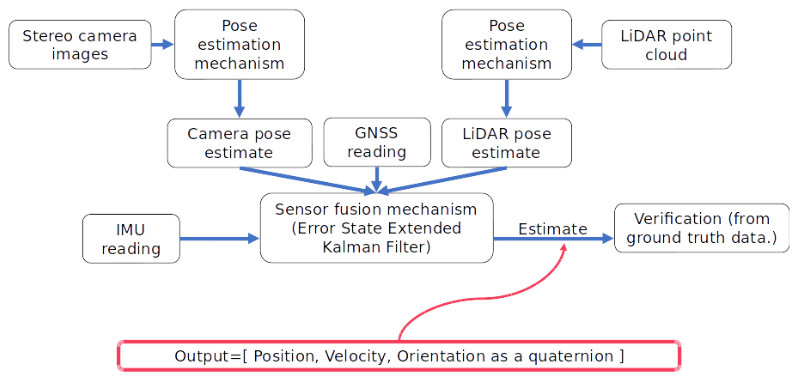
\includegraphics[width=\textwidth]{figs/system-block-diagram.png}
	\end{center}
	\vspace{-0.5cm}
	\caption{System block diagram}
	\label{fig:pa:systemBlockDiagram}
	\vspace{0.5cm}
\end{figure}

The system is implemented on \gls{ROS}, along with evaluation and visualization mechanisms for demonstrating functionality. Main programming language used is Python. Each of the components mentioned in the above discussion will be explained in detail, in the subsequent sections.







%%%%%%%%%%%%%%%
\section{Coordinate frames}
Apart from each sensor's own coordinate frame, in which they provide measurements, we define the following coordinate frames which will be used in the rest of this report.\\\\
\begin{tabular}{p{0.2\linewidth} p{0.75\linewidth} } 
	Inertial frame & An earth fixed right-handed rectilinear coordinate frame with x, y and z axes pointing towards East, North and Up directions respectively(ENU frame). The origin of the frame is determined by the information given in the dataset being used.\\\\
	Body frame & A right-handed rectilinear coordinate frame fixed to the vehicle with x, y and z directions pointing lateral, front and upward directions of the vehicle respectively.
\end{tabular}\\\\
Figure \ref{fig:pa:coordinateFrames} illustrates the above-mentioned coordinate frames.
\begin{figure}[h]
	\begin{center}
	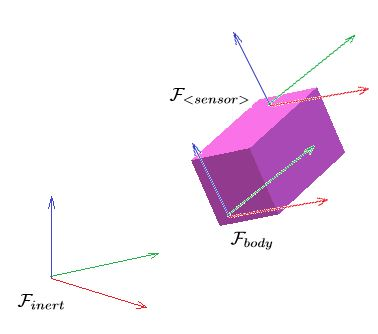
\includegraphics[width=0.6\textwidth]{figs/coordinate-frames.jpg}
	\end{center}
	\vspace{-0.5cm}
	\caption[Coordinate frames]{Illustration of the coordinate frames. x, y and z axes of each coordinate frame is depicted in red, green and blue colours, respectively. The cuboid represents the vehicle. The sensor is assumed to be mounted on the front side of the roof of the vehicle.}
	\label{fig:pa:coordinateFrames}
	\vspace{0.5cm}
\end{figure}






%%%%%%%%%%%%%%%%
\section{Datasets}
We have been using three public datasets, namely, \gls{NCLT} dataset\cite{pa:NCLTDataset}, \gls{KITTI} dataset for tracking\cite{pa:KITTIDataset} and \gls{KAIST} Urban dataset\cite{pa:KAISTDataset}. In addition, we expect to use the EU-Long Term dataset\cite{pa:EULTDataset}. All these datasets include data from sensors that are sufficient for the sensor fusion mechanism, along with ground truth data. Details of the datasets are given in table \ref{table:pa:Datasets}.
% TODO: dataset info table
\begin{table}[h]
\centering
\begin{tabular}{ |p{0.1\textwidth}|p{0.27\textwidth}|p{0.2\textwidth}|p{0.10\textwidth}|p{0.18\textwidth}|  }
	\hline
	\textbf{Dataset} & \textbf{Sensors} & \textbf{Ground truth} & \textbf{Distance} & \textbf{Data Format}\\
	\hline
	KITTTI  & $1\times$ $64$-layer LiDAR \newline $2\times$ grayscale camera \newline $2\times$ stereo camera \newline $1\times$ GPS-RTK/INS & scene flow, odometry object detection and tracking, road and lane&  $39.2$ km & png (camera) \newline txt(GPA-RTK/INS) \newline bin (LiDAR)\\
	\hline 
	KAIST & $2\times$ $16$-layer LiDAR \newline $2\times$ $1$-layer LiDAR\newline $2\times$ monocular camera\newline $1\times$ consumer-level GPS\newline $1\times$ GPS-RTK\newline $1\times$ fiber optic gyro\newline $1\times$ independant IMU\newline $2\times$ wheel encoder\newline $1\times$ altimeter & SLAM algorithm for vehicle self-localization &$190.989$ km & bin(LiDAR)\newline png(camera)\newline csv(GPS-RTK/IMU)\\
	\hline
	NCLT & $1\times$ $32$-layer LiDAR\newline $2\times$ planar LiDAR\newline $1\times$ camera\newline $1\times$ independant IMU\newline$1\times$ fibre optic gyro\newline $1\times$ consumer-level GPS\newline $1\times$ GPS-RTK\newline & SLAM algorithm for vehicle self-localization with GPS-RTK &$147.4$ km & tiff(image)\newline csv(GPS-RTK/IMU)\newline bin(LiDAR)\\
	\hline
	EU-Long Term & $2\times$ $32$-layer LiDAR\newline $1\times$ $4$-layer LiDAR\newline $1\times$ $1$-layer LiDAR\newline $2\times$ stereo camera \newline $2\times$ fisheye camera\newline $1\times$ radar\newline $1\times$ GPS-RTK\newline $1\times$ independant IMU\newline & GPS-RTK/IMU for vehicle self-localization & $63.4$ km & rosbag (All-in-one)\\
	\hline
\end{tabular}
\caption{Dataset information}
\label{table:pa:Datasets}
\end{table}







%%%%%%%%%%%% ch start %%%%%%%%%%%

\section{Comparison of Bayesian filters}
Kalman Filters are the most widely used sensor data fusion algorithms. There 
are many extensions to the basic Kalman Filter (which is known as the Linear Kalman Filter), allowing them to be used in variety of applications. Table \ref{table:ch:KalmanFilterComparison} provides a 
comparison between different types of Kalman filters. Note that the computational complexity of the filters increases from left to right.
\begin{table}[h]
	\centering
	\begin{tabular}{|p{3.4cm}|p{3.4cm}|p{3.4cm}|p{3.4cm}|} 
		\hline
		% \textbf{Linear Kalman} & \textbf{Extended Kalman} & \textbf{Error State} & \textbf{Unscented} \\
		% \textbf{Filter} & \textbf{Filter} & \textbf{Kalman Filter} & \textbf{Kalman Filter} \\
		\textbf{Linear Kalman Filter} & \textbf{Extended Kalman Filter} & \textbf{Error State Extended Kalman Filter} & \textbf{Unscented Kalman Filter} \\
		\hline
		Linear Gaussian model&Non-linear Gaussian model&Non-linear  Gaussian model&Non-linear Gaussian model\\
		\hline
		Best linear unbiased estimator (Blue)&Linearize the nonlinear dynamics using Jacobeans (Taylor series)&Linearize the nonlinear 
		dynamics of error using Jacobeans (Taylor series)&Calculate sigma points and use Unscented Transform to approximate the \gls{PDF}s directly\\
		\hline
		Estimates the state & Estimates the state& Estimates the error of the state & Estimates the state\\
		\hline
	\end{tabular}
	\caption{Comparison of different types of Kalman Filters}
	\label{table:ch:KalmanFilterComparison}
\end{table}

Kalman Filters can only be used for Gaussian models. However, we cannot use the Linear Kalman Filter at all because the localization task is not linear. Assuming that the localization problem is Gaussian, other Kalman Filters can be used to tackle the problem. We selected  \gls{UKF} and \gls{ESKF} to implement in python since those two algorithms have shown the best results among Kalman filters according to \cite{ch24:st2004comparison},\cite{ch25:madyastha2011extended} and \cite{ch26:wan2000unscented}.

\gls{PF} was recently suggested after \gls{KF}s to process arbitrary inertial sensor characteristics, motion dynamics, and noise distributions. When dealing with non-linear models in motion equations and measurement relations with a non-Gaussian noise assumption, the Kalman Filter methods may lead to non-optimal solutions. However, particle filters provide general solutions to many problems where linearization and Gaussian approximations are intractable \cite{ch27:ababsa2004comparison}. A brief comparison of \gls{PF}s and \gls{KF}s is given in Table \ref{table:ch:KFandPFComparison}.
\begin{table}[h]
\centering
	\begin{tabular}{|c|c|} 
		\hline
		\textbf{Kalman Filters} & \textbf{Particle Filters} \\
		\hline
		Only for Gaussian models & For both Gaussian and non-Gaussian models\\
		\hline
		Only for linear models& For both linear and non-linear models
		\\
		\hline
		Low computational complexity&High computational complexity\\
		\hline
	\end{tabular}
	\caption{A brief comparison of Kalman Filters and Particle Filters}
	\label{table:ch:KFandPFComparison}
\end{table}

Three basic level filters (namely, \gls{PF}, \gls{ESKF}, and \gls{UKF}) were implemented and compared using the \gls{NCLT} data set to select the best filter for our application. Afterwards, the performance of the  best filter was improved by increasing the number of elements in the state vector, adding \gls{ZUPT} measurements, and fusing relative measurements (visual and \gls{LiDAR} odometry) etc. The state vector used for the basic filter implementations was
\begin{align}
\label{eq:ch:basicStateVector}
   \textbf{x} &= \left[\begin{matrix}{}\textbf{p}\\\textbf{v}\\\textbf{q}\end{matrix}\right]
\end{align}
where,
\begin{align}
	\textbf{p}&=(p_x,p_y,p_z) \text{ position relative to the inertial frame}\\
	\textbf{v}&=(v_x,v_y,v_z) \text{ velocity relative to the inertial frame}\\
	\textbf{q}&=(q_\omega,q_x,q_y,q_z) \text{ quaternion relative to the inertial frame}.
\end{align}

The \gls{ESKF} estimates the error state directly and uses it as a correction to the nominal state. Number of particles used in the \gls{PF} was 1000. Gaussian random noise was added to the particles before applying the motion model, to increase the diversity of the particles. Systematic Resampling was used to resample particles when needed and squared error function was used as the weight function. Following values were selected for the parameters (as defined in \cite{ch26:wan2000unscented}) of the \gls{UKF};
\begin{align}
	\alpha &= 1 \text{ (determines the spread of sigma points)}\\
	\beta & = 2 \text{ (used to incorporate prior knowledge of the \gls{PDF} of the state)}\\
	k &= 1 \text{ (a secondary scaling factor, similar to $\alpha$)}.
\end{align}

Based on the results obtained (see section \ref{sec:BayesianFilterComparison}), \gls{ESKF} was selected as the best filter to tackle our problem.


%%%%%%%%%%%% ch end %%%%%%%%%%%%%







%%%%%%%%%%%%%%%
\section{Sensor fusion mechanism}
\subsection{The \acrlong{ES-EKF}}
The \gls{ES-EKF} acts as the component responsible for fusing sensor data. As mentioned in section \ref{sec:SystemArchitecture}, our \gls{ES-EKF} currently has 16 nominal state space variables and 15 error state space variables, grouped into 5 sub-vectors, as listed below;
\begin{align}
    \text{Nominal state vector: }\textbf{x} &= \left[\begin{matrix}{}\textbf{p}\\\textbf{v}\\\textbf{q}\\\boldsymbol{a_b}\\\boldsymbol{\omega_b}\end{matrix}\right]
\end{align}
where
\begin{align}
    \textbf{p} &= (p_x, p_y, p_z) \text{ position relative to the inertial frame} \nonumber \\
    \textbf{v} &= (v_x, v_y, v_z) \text{ velocity relative to the inertial frame} \nonumber \\
    \textbf{q} &= (q_w, q_x, q_y, q_z) \text{ quaternion relative to the inertial frame} \nonumber \\
    \boldsymbol{a_b} &= (a_{bx}, a_{by}, a_{bz}) \text{ acceleration biases of the IMU relative to the body frame} \nonumber \\
    \boldsymbol{\omega_b} &= (\omega_{bx}, \omega_{by}, \omega_{bz}) \text{ angular velocity biases of the IMU relative to the body frame}
\end{align}
and
\begin{align}
	\text{Error state vector: }\boldsymbol{\delta}\textbf{x} &= \left[\begin{matrix}{}\boldsymbol{\delta}\textbf{p}\\\boldsymbol{\delta}\textbf{v}\\\boldsymbol{\delta}\boldsymbol{\theta}\\\boldsymbol{\delta}\boldsymbol{a_b}\\\boldsymbol{\delta}\boldsymbol{\omega_b}\end{matrix}\right].
\end{align}
Here, $\boldsymbol{\delta}\boldsymbol{\theta}$ is the error in orientation, expressed as an axis-angle vector. Furthermore, $\boldsymbol{\delta}\boldsymbol{a_b}$ and $\boldsymbol{\delta}\boldsymbol{\omega_b}$ are the considered as global errors. The motion model for the prediction step of the filter is given below.\\
Nominal state update:
\begin{align}
    \check{\textbf{p}}_k &= \hat{\textbf{p}}_{k-1}+\hat{\textbf{v}}_{k-1}\Delta t + \frac{1}{2} \left( \textbf{R}_{inert,body}\left(\textbf{a}_{m_{k-1}}-\hat{\textbf{a}}_{b_{k-1}}\right)+\textbf{g}\right)\Delta t^2 \\
    \check{\textbf{v}}_k &= \hat{\textbf{v}}_{k-1}+\left(\textbf{R}_{inert,body}\left(\textbf{a}_{m_{k-1}}-\hat{\textbf{a}}_{b_{k-1}}\right)+\textbf{g}\right)\Delta t \\
    \check{\textbf{q}}_k &= \hat{\textbf{q}}_{k-1}\otimes \textbf{q}\left\{\left(\boldsymbol{\omega}_{m_{k-1}}-\hat{\boldsymbol{\omega}}_{b_{k-1}}\right)\Delta t\right\} \\
    \check{\textbf{a}}_{b_k} &= \hat{\textbf{a}}_{b_{k-1}} \\
    \check{\boldsymbol{\omega}}_{b_{k}} &= \hat{\boldsymbol{\omega}}_{b_{k-1}}
\end{align}
with
\begin{align}
	\textbf{a}_{m_{k}} &= \text{Acceleration measured by accelerometer at k\textsuperscript{th} instance}\\
	\boldsymbol{\omega}_{m_{k}} &= \text{Angular velocity measured by gyroscope at k\textsuperscript{th} instance}\\
    \textbf{R}_{inert,body} &= \text{Rotation matrix corresponding to $\hat{\textbf{q}}_{k-1}$} \\
	\textbf{g} &= \text{Gravity vector w.r.t inertial frame}\\
	\otimes &= \text{Quaternion composition operator.}
\end{align}
Error state covariance matrix update:
\begin{align}
    \Check{\textbf{P}}_k &= \textbf{F}_x\hat{\textbf{P}}_{k-1}\textbf{F}_x^T + \textbf{F}_i\textbf{Q}_i\textbf{F}_i^T
\end{align}
where
\begin{align}
	\textbf{P}_k &= \text{Error state covariance matrix at k\textsuperscript{th} instance}\\
	\textbf{F}_x &= \left.\frac{\partial f}{\partial \boldsymbol{\delta}\textbf{x}}\right|_{\textbf{x}=\hat{\textbf{x}}_{k-1} , \boldsymbol{\delta}\textbf{x}=\textbf{0} , \textbf{w}=\textbf{0}}\\
	\textbf{F}_i &= \left.\frac{\partial f}{\partial \textbf{w}}\right|_{\textbf{x}=\hat{\textbf{x}}_{k-1} , \boldsymbol{\delta}\textbf{x}=\textbf{0} , \textbf{w}=\textbf{0}}\\
	f(.) &= \text{Function representing the motion model}\\
	\textbf{w} &= \text{Process noise vector}\\
	\textbf{Q}_i &= \text{Process noise covariance matrix}.
\end{align}
The equations pertaining to the correction process, upon receiving a measurement update is given below.
\begin{align}
    \textbf{K}_k &= \check{\textbf{P}}_k\textbf{H}^T\left(\textbf{H}\check{\textbf{P}}_k\textbf{H}^T+\textbf{V}\right)^{-1} \\
    \hat{\textbf{P}}_k &= \left(\textbf{I}-\textbf{K}_k\textbf{H}\right)\check{\textbf{P}}_k\\
	\hat{\boldsymbol{\delta}\textbf{x}_k} &= \textbf{K}_k \left(\textbf{y}-h\left(\check{\textbf{x}}_k\right)\right)\\
	\hat{\textbf{x}}_k &= \check{\textbf{x}}_k \oplus \hat{\boldsymbol{\delta}\textbf{x}}_k\\
	\hat{\boldsymbol{\delta}\textbf{x}}_k & \leftarrow \textbf{0}.
\end{align}
Here,
\begin{align}
	h(.) &= \text{Measurement function}\\
	\textbf{H} &= \text{Jacobian of the measurement function, relative to the error state,}\nonumber\\
	&\quad\text{ evaluated at zero}\\
	\textbf{V} &= \text{Measurement noise matrix}\\
	\textbf{y} &= \text{Measurement vector}\\
	\textbf{I} &= \text{Identity matrix of suitable dimension}\\
	\oplus &= \text{Operator representing the combination of nominal state and error state }\nonumber\\
	&\quad\text{ vectors}.
\end{align}
For a detailed presentation of the matrices involved in above equations, refer Appendix \ref{appendix:ESEKFMatrices}\cite{pa:Sola2017QuaternionKinematics}.


\subsection{Stochastic cloning and backward smoothing}
Following the works of Emter et. al\cite{pa:Emter2018StochasticCloning},  we have implemented a stochastic cloning framework along with the \gls{ES-EKF}, as a mean of integrating relative measurements obtained from sensors such as wheel odometer and visual/\gls{LiDAR} odometry algorithms. Since a relative measurement relates the current state of the vehicle to a previous state, it is required to propagate the corrections resultant from absolute measurements to all the previous states as well. In-order to achieve this, a \gls{RTS} backward smoother was integrated.


\subsection{State buffer}
It is essential to store a window of previous estimates obtained as the output of the \gls{ES-EKF}, in-order to be used when fusing a relative measurement, under stochastic cloning framework. A buffer with predefined length was implemented to achieve this functionality. Once a prediction is done by the \gls{ES-EKF}, the estimate is added to the buffer. If the buffer is full, the oldest estimate will be removed, keeping the buffer length a constant.

Other than the estimate itself, the motion model inputs that resulted the prediction of the estimate and the prediction covariance matrix are also stored in this buffer. In addition to the stochastic cloning mechanism, they are used in propagating the effect of an absolute measurement correction across all the states of the buffer.

\subsection{Time synchronization}
Measurements from different sensors arrive at different times, in different rates. These asynchronous arrivals are handled using the \gls{ROS}'s in-built multi-threading behaviour of subscriber callback functions. Each sensor publishes data to its own \gls{ROS} topic, for which the localization module is subscribed to. Hence, each publication will invoke a callback function, which includes the logic for carrying out either a prediction or a correction step, depending on the measurement received.

When an absolute correction is to be carried out, the filter first searches the state buffer, for the state with the closest timestamp to that of the measurement. Then it performs correction steps on that state. After it has been completed, the effect of the correction has to be propagated to all the remaining states in the buffer. States having later timestamps will be adjusted by re-predicting them based on the corrected state. States with earlier timestamps will be adjusted through performing \gls{RTS} smoothing. A similar procedure is carried out upon receiving a relative measurement, except that, backward smoothing with \gls{RTS} will not be performed.

In this manner, a delayed measurement can still contribute to a correction, unless it is too delayed, so that the state corresponding to its timestamp no longer exists in the state buffer.

If a prediction is to be carried out, the filter will only search for the latest timestamp of the states. If it is greater than that of the prediction input, the input will be neglected. Otherwise, a prediction will be carried out and the newly predicted state will be added to the state buffer.

% TODO: add image illustrating time synchronization


\subsection{\acrlong{ZUPT} measurements}
Some of the physical constraints that govern the motion of a vehicle can be incorporated into the sensor fusion mechanism, in-order to make the estimate more accurate. \gls{ZUPT} measurements, generated based on the fact that the motion of a vehicle is constrained only towards its longitudinal direction, are one such constraint that can be employed to couple the positional measurements with the heading estimation \cite{pa:Dissanayake2001ZUPT}. 

However, it should be noted that, the advantages of \gls{ZUPT} measurements come at a cost. Since they are fed into the \gls{ES-EKF} as ordinary absolute measurements, they reduce the estimated covariance of the error, causing the filter to be overconfident on its estimate. Furthermore, once diverged due to erroneous measurements, the estimate takes a longer time to converge back to the ground truth, after starting to receive correct measurements. These effects should be balanced out by carefully tuning the noise variance of the \gls{ZUPT} measurement.






%%%%%%%%%%%%%%%% ra start %%%%%%%%%%%%%%%%%%

\section{Visual Odometry}
Out of the sensors that we use for localization process, cameras are the cheapest. However, it is capable of providing rich information of the environment, which allows us to recognize the environment robustly and accurately. Therefore, camera based visual odometry \gls{SLAM} solutions are becoming very popular, and can be used in our system as a solution for \gls{GNSS} outages. 

\subsection{System Selection}
\label{subsec:vodomSystemSelection}
Monocular camera based systems are the most commonly used for visual odometry because of the low cost and the smaller sensor setup. However, estimations are not reliable and inaccurate because depth cannot be calculated using one camera \cite{ra:ORB_SLAM2}. Therefore, stereo camera based systems were selected as the best solution for our system. As implementation of this algorithm was not within the project scope, we had to find a solution with an existing implementation. Following criteria were used when selecting a suitable method:
\begin{itemize}
    \item Should not depend on previously generated feature maps
    \item Should provide real time output
    \item Accuracy
    \item Availability of proper implementation
\end{itemize}

\gls{ORBSLAM} \cite{ra:ORB_SLAM2} and \gls{S-PTAM} \cite{ra:S-PTAM} were the best solutions available. Furthermore, they had proper implementations, available for free. Comparing the results they have obtained by testing these algorithms using the KITTI dataset \cite{ra:KITTI}, \gls{ORBSLAM} showed superior perfomance over \gls{S-PTAM}. Furthermore, the implementation of the \gls{ORBSLAM} algorithm was fairly detailed. Hence, we selected \gls{ORBSLAM} as the best solution.


\subsection{\gls{ORBSLAM} algorithm}
This is an extension of the previously implemented \gls{ORBSLAM} algorithm \cite{ra:ORB_SLAM}, which was only for the monocular systems. In the \gls{ORBSLAM}, they have extended the previous implementation for the stereo cameras with accuracy improvements\cite{ra:ORB_SLAM2}. 
\begin{figure}[t]
	\centering
	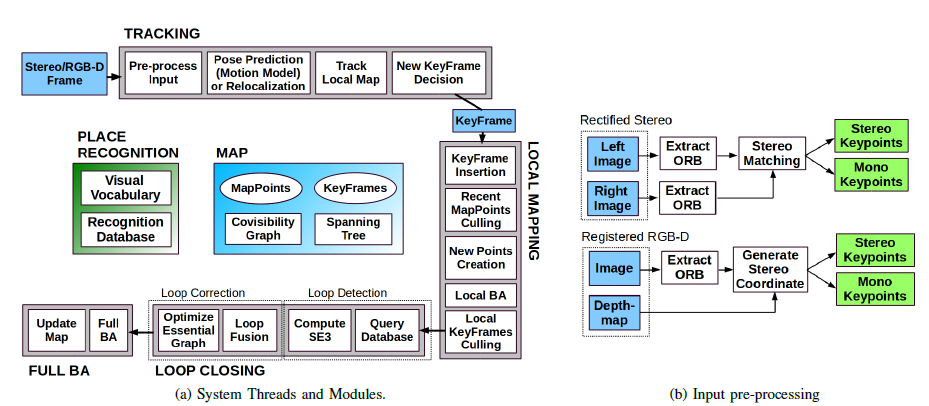
\includegraphics[width=\textwidth]{figs/ORB_SYSTEM.png}
	\vspace{-0.5cm}
	\caption{\gls{ORBSLAM} architecture \cite{ra:ORB_SLAM2}}
	\label{fig:ra:ORB_SYSTEM}
	\vspace{0.5cm}
\end{figure}

Pre-processing architecture is shown in figure \ref{fig:ra:ORB_SYSTEM}(b). Features of the rectified stereo images will be extracted using the ORB feature extractor \cite{ra:ORB} and extracted features will be matched with the previous frame to identify the stereo key points. 

General view of the system architecture is shown in figure \ref{fig:ra:ORB_SYSTEM}(a). System is consisted of three main parallel threads, namely;
\begin{enumerate}
	\item the Tracking thread to localize the camera with every frame by finding feature matches to the local map and minimizing the re-projection error applying motion-only \gls{BA}
	\item the Local Mapping thread to manage the local map and optimize it, performing local BA\gls{BA}
	\item the Loop Closing thread to detect large loops and correct the accumulated drift by performing a pose-graph optimization \cite{ra:ORB_SLAM2}.
\end{enumerate} 

In the existing code, the vehicle is localized on a local map created using the feature points. However, for our system, we needed to get the relative transform of the vehicle, between two stereo frames. Hence, we modified the existing algorithm to receive relative transform of the vehicle, directly, as the output. The result is published as a ROS\gls{ROS} message.

\gls{ORBSLAM} has been designed and setup only for the \gls{KITTI} and \gls{TUM} datasets. We added the image rectification functionality for the \gls{KAIST}, as we will be using that dataset for our testing purposes.

One drawback of the \gls{ORBSLAM} algorithm is the absence of a reliability metric (eg: estimated variance of the error) for the estimate. In order to circumvent this problem, we have been testing different methods to obtain an error covarince matrix. One of the methods tested was to estimate covariance values based on the number of features matched between each pair of frames. We hypothesized that the error should be reduced if a higher number of features have been detected. However, this hypothesis has been observed to be invalid (see section \ref{sec:VisualOdometry}). Hence, alternatives are being sought to overcome this issue. 

%%%%%%%%%%%%%%%% ra end %%%%%%%%%%%%%%%%%%%%








%%%%%%%%%%%%%%%% hi start %%%%%%%%%%%%%%%%%%


\section{Lidar Odometry}
In vehicle localization, out of the sensors that we use, \gls{LiDAR} is the most expensive and accurate sensor. It is capable of providing point clouds of the surrounding environment (well-defined rich information) which allows us to recognize the environment robustly and accurately. 360-degree feature space exploration is the best advantage that we can gain from a high-end \gls{LiDAR}, which we can’t obtain with cameras and other sensors regardless of their quality. However, this elevated accuracy comes at a significantly higher cost, relative to the rest of the sensors.

\subsection{Method Selection}
As implementation of a \gls{LiDAR} odometry algorithm is not within the scope of this project, we had to find a solution with an existing implementation. The criteria followed in this selection was similar to that as in the case of visual odometry algorithm (see section \ref{subsec:vodomSystemSelection}). 
\begin{table}[h]
	\centering
	\begin{tabular}{|p{0.3\textwidth}|p{0.3\textwidth}|p{0.15\textwidth}|p{0.15\textwidth}|} 
		\hline
		\textbf{Algorithm} & \textbf{Features} & \textbf{Complexity} & \textbf{Robustness} \\
		\hline
		Conventional \gls{ICP}&Accuracy mainly depends on the correspondence
		matching&Low&Low\\
		\hline
		\gls{NDT}&No correspondence feature matching&Moderate&Moderate\\
		\hline
		\gls{LOAM}&IMU data makes estimation more robust& High & High\\
		\hline
		\gls{LeGO-LOAM}&IMU data makes estimation more robust& High & Very High\\
		\hline
	\end{tabular}
	\caption{Different \gls{LiDAR} odometry algorithms}
	\label{table:ha:DifferentLOdomMethods}
\end{table}

\gls{LOAM} \cite{hi:LOAM} and the \gls{LeGO-LOAM} \cite{hi:LeGO-LOAM} were the best solutions that we found with a proper implementation in the literature. Comparing the benchmark errors received by testing the algorithms using the \gls{KITTI} dataset, \gls{LeGO-LOAM} showed the better estimation. Depending on the results, along with the comparison presented in table \ref{table:ha:DifferentLOdomMethods}, we selected the \gls{LeGO-LOAM} as the best solution for our localization module.

\subsection{\gls{LeGO-LOAM}}
\gls{LeGO-LOAM} algorithm is an extension of the \gls{LOAM} algorithm with new features added to make it more accurate, robust and fast in terms of computation. Following list presents some such modifications.
\begin{itemize}
    \item Project the \gls{LiDAR} points into a range image 
    \item Segment the ground plane and separate the ground plane from the image
    \item Apply image based segmentation method (clustering) to extract separate clusters
    \item Feature extraction phase is more robust and fast since feature extraction is carried out with segmented objects and planes, rather than raw points, as in \gls{LOAM}.
\end{itemize}

\begin{figure}[t]
	\centering
	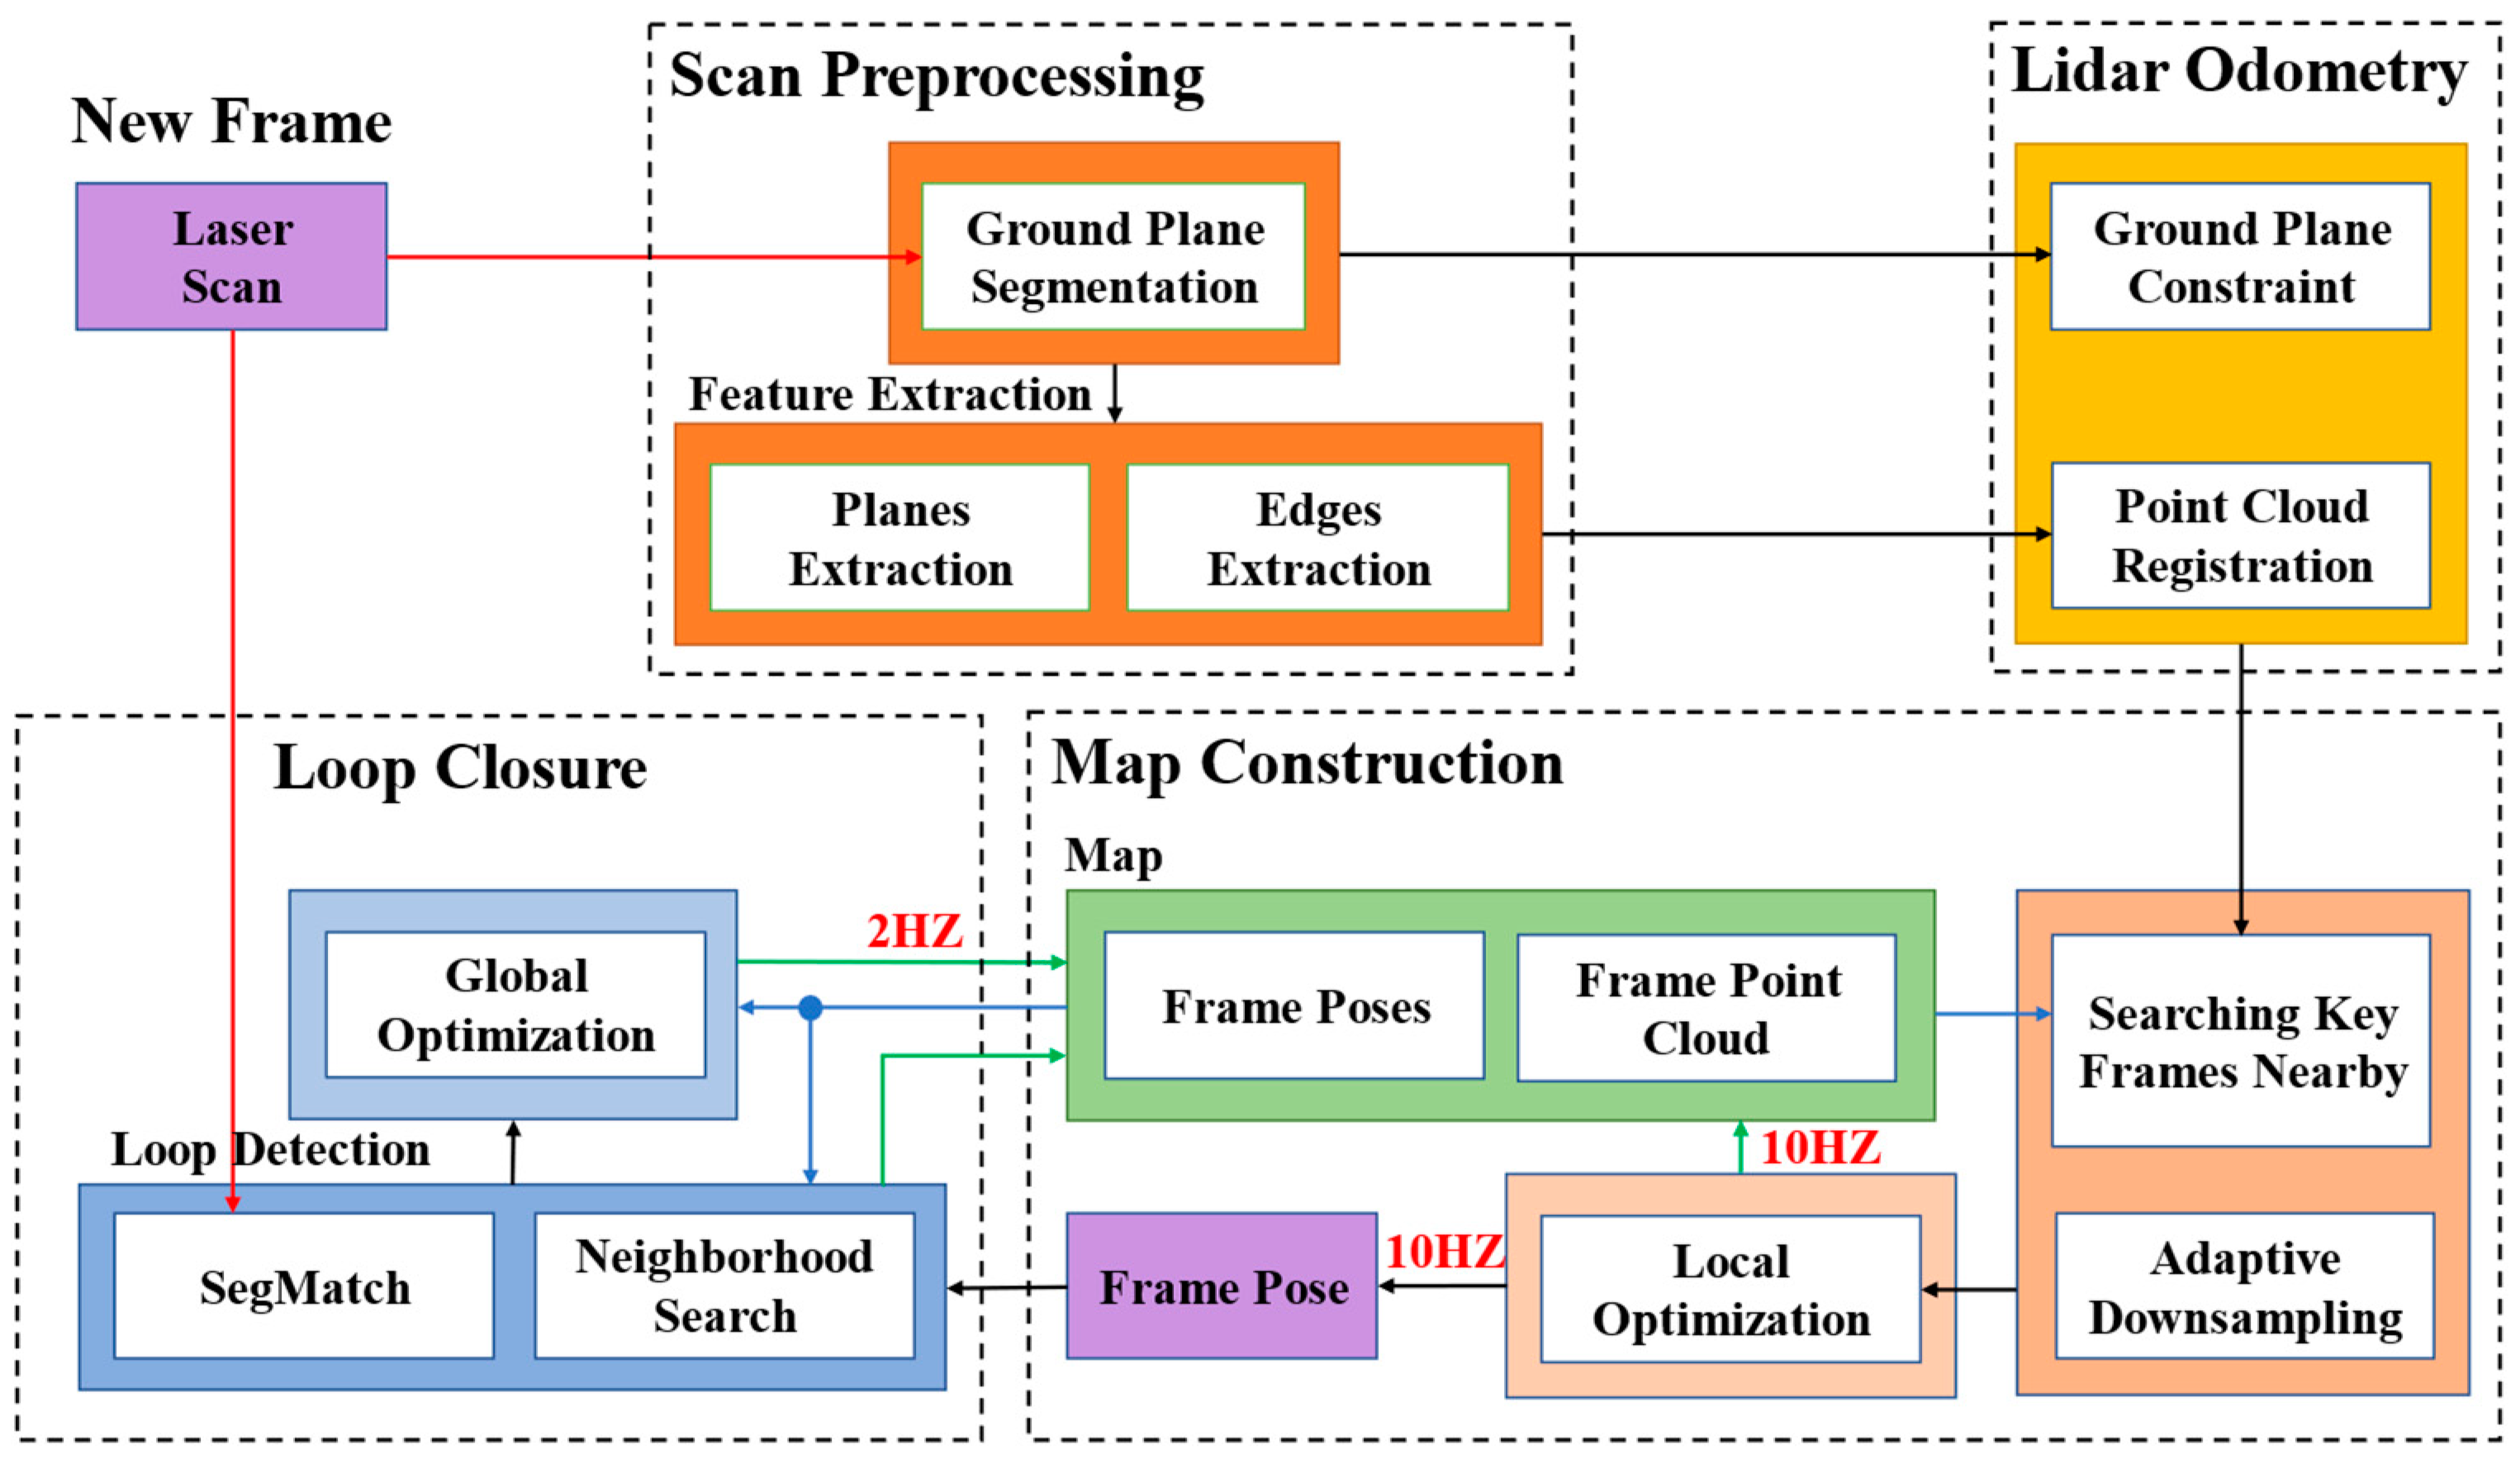
\includegraphics[ width=\textwidth]{figs/loam_architect.png}
	\vspace{-0.5cm}
	\caption{ \gls{LeGO-LOAM} system architecture\cite{hi:LeGO-LOAM}}
	\label{fig:hi:LeGO_LOAM_SYSTEM}
	\vspace{0.5cm}
\end{figure}

General view of the \gls{LeGO-LOAM} system architecture is shown in figure \ref{fig:hi:LeGO_LOAM_SYSTEM}. System consists of four main modules; scan preprocessing, odometry, map construction and global optimization. Scan preprocessing module projects the \gls{LiDAR} points onto a range image, segments the ground plane and separate the ground plane from the image. Then it applies image based segmentation methods for ground plane segmentation and edge features  are extracted from the projected image. Odometry module takes care of feature matching and transformation optimization for \gls{LiDAR} point cloud registration and generates odometry measurement. Map construction module uses the previous key frames and odometry estimation to construct the map and also adds fast optimization to the odometry estimation. Loop closure module adds global optimization and drift correction to the map and makes the construction much more drift free.

In the existing code, the vehicle is localized on a local map created using the map construction module. However, for our system, we need to get the relative transform of the vehicle as an output. Therefore, the adjustments have been made to the existing algorithm to receive relative transform of the vehicle for every \gls{LiDAR} scan.

The issue of not having a mechanism to obtain the covariance of the pose-estimate error is a limitation of this algorithm, as well. Hence, we expect to find solutions for this issue based on metrics such as the final optimized error in \gls{LM} algorithm \cite{hi:LM_optimization} etc.


%%%%%%%%%%%%%%%% hi end %%%%%%%%%%%%%%%%%%%%










%%%%%%%%%%%%%%%%
\section{Implementation on \acrlong{ROS}}
The system was implemented on \gls{ROS}, targetting the easy integration with other modules (path planning, perception etc.) of the autonomous vehicle. Furthermore, the \gls{ROS} environment facilitates the following;
\begin{itemize}
	\item Visualizing results (through Rviz, Multiplot etc.)
	\item In-built multi-threading for handling asynchronous data feeds
	\item Controlling simulation time
	\item Inter-process communication through \gls{ROS} topics
	\item Debugging (using tools such as Node Graphs, TF Tree etc.)
	\item Handling transformations (through TF)
\end{itemize}
Apart from the nodes for visual and \gls{LiDAR} odometry algorithms, the system consists of 3 main nodes, namely, the Data Feeder, Locator and the Evaluator. Each of these nodes will be described separately, in the following discussion. Figure \ref{fig:pa:nodeGraph} shows the Node Graph obtained for the system.

\begin{figure}[h]
	\begin{center}
	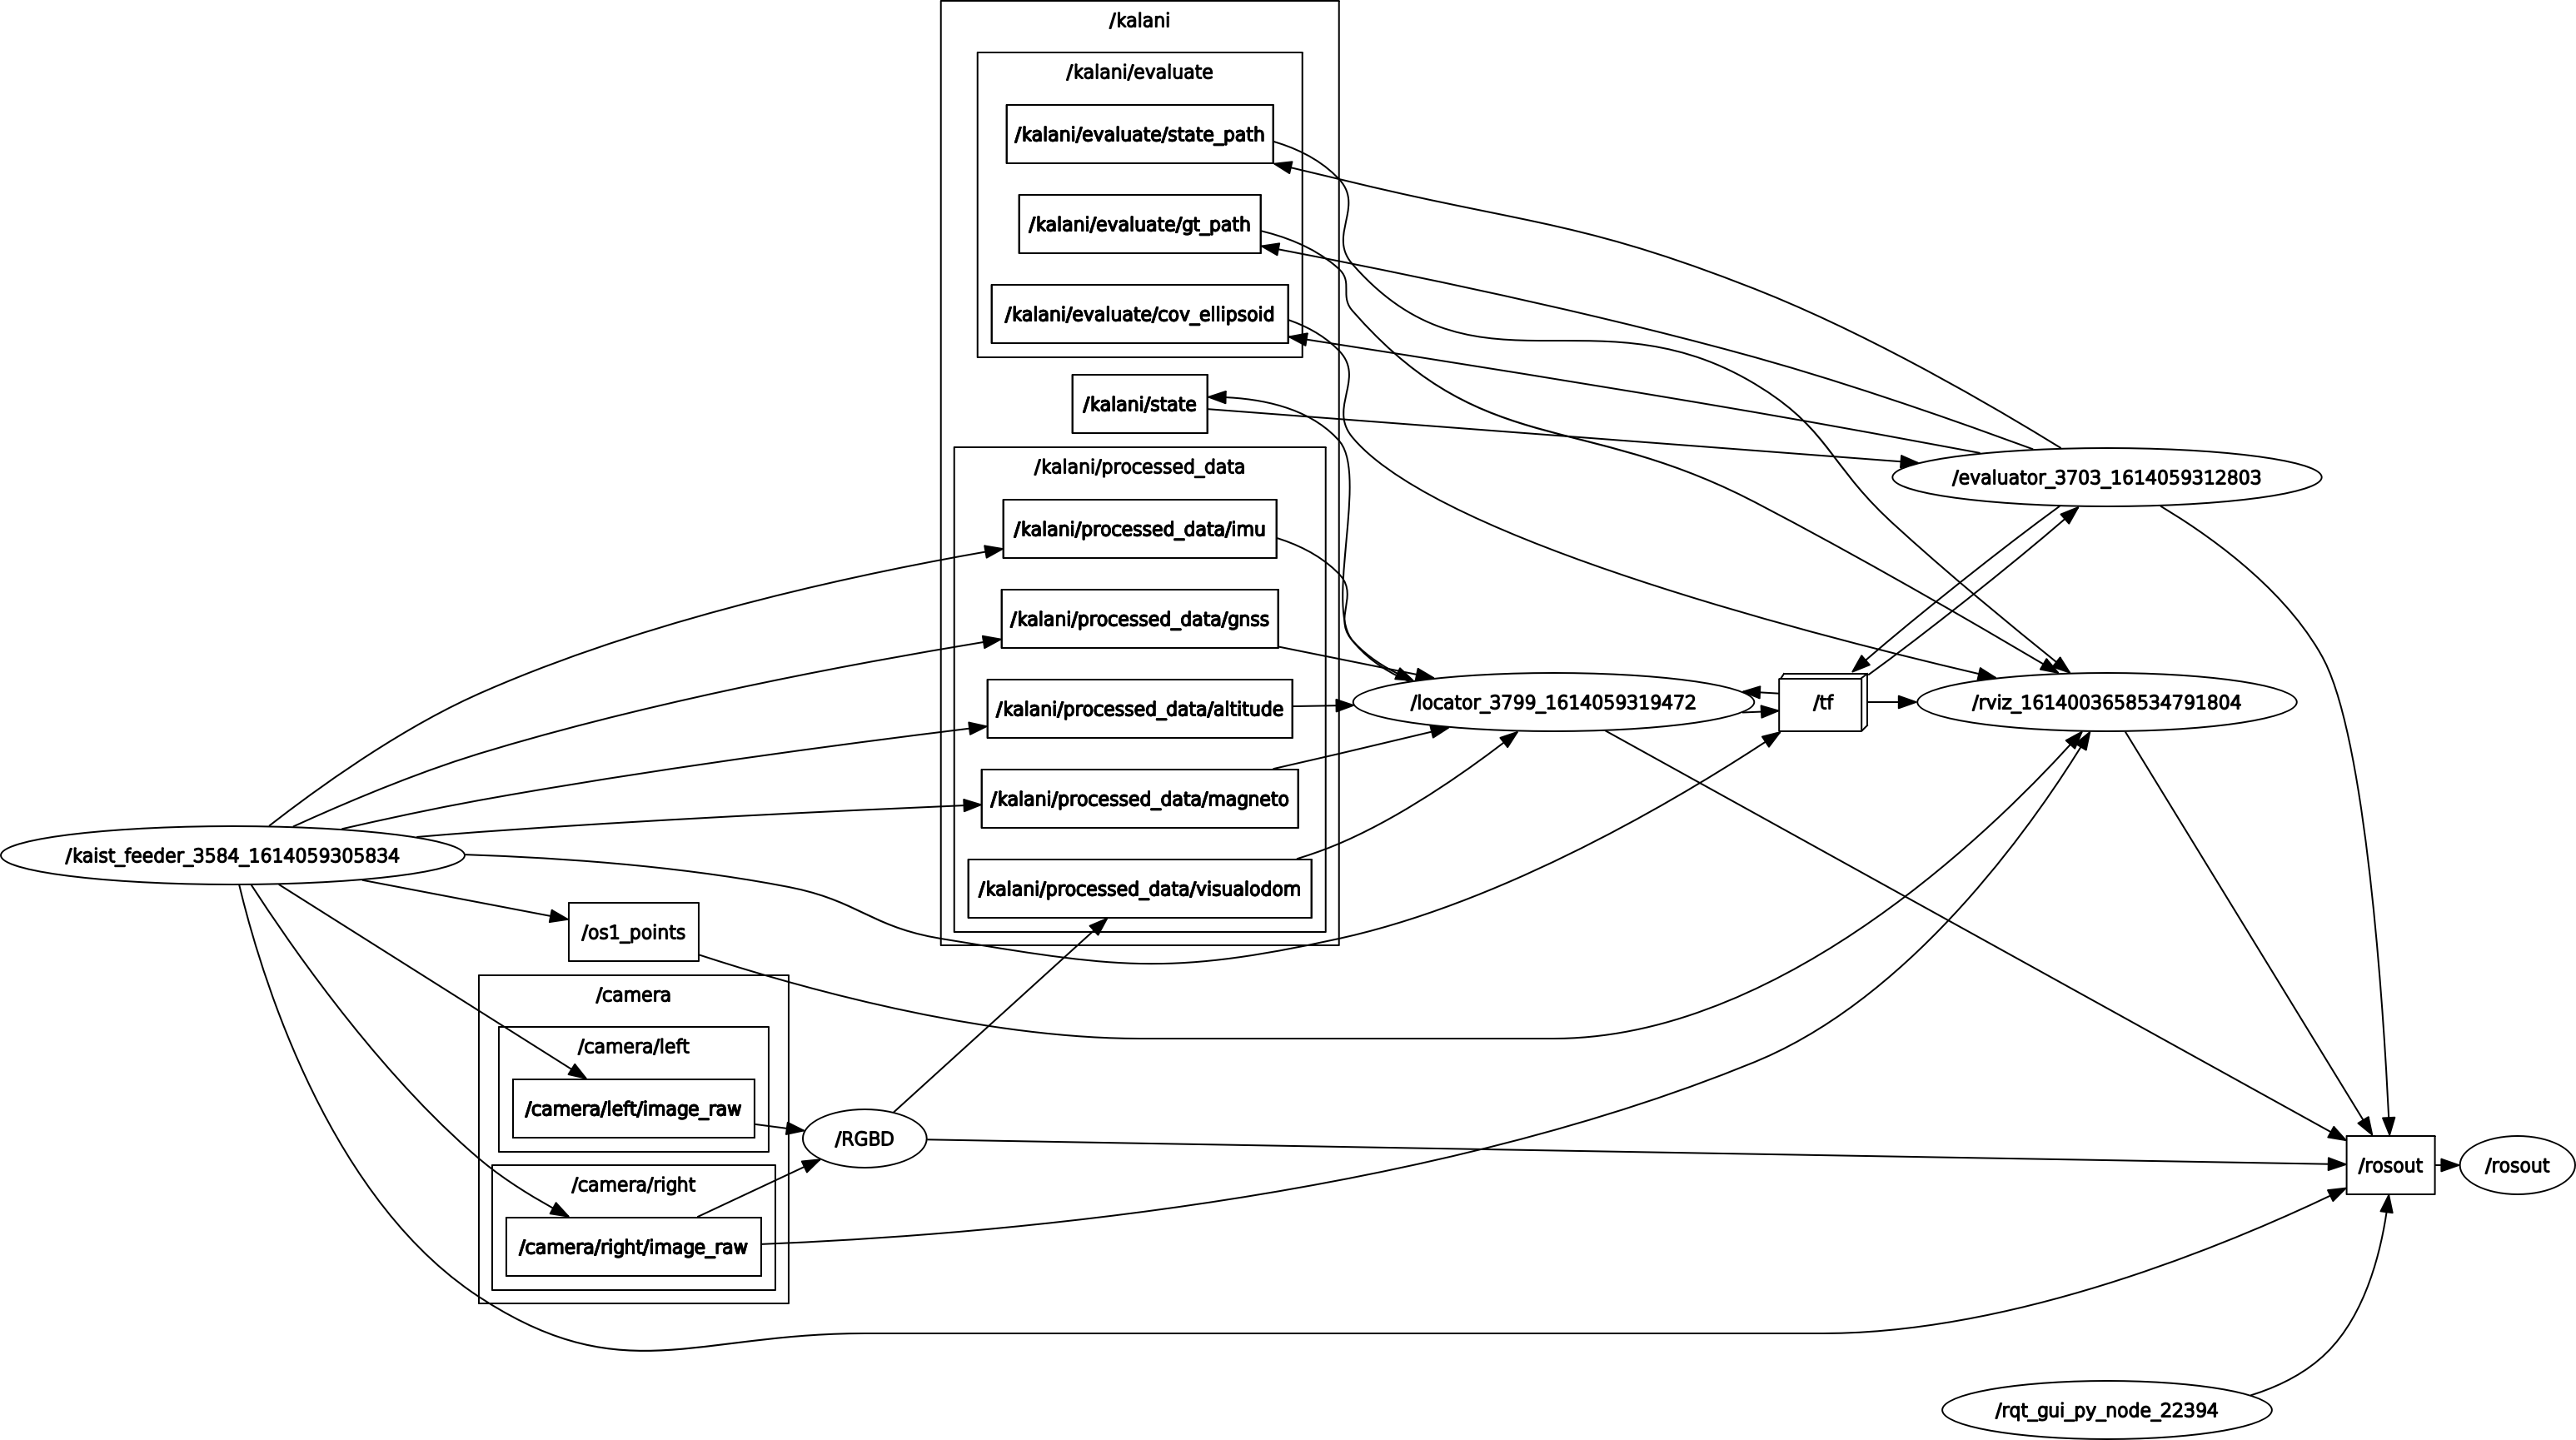
\includegraphics[width=\textwidth]{figs/rosgraph.png}
	\end{center}
	\vspace{-0.5cm}
	\caption[\gls{ROS} Node Graph]{\gls{ROS} Node Graph}
	\label{fig:pa:nodeGraph}
	\vspace{0.5cm}
\end{figure}

\subsection{Data Feeder}
This \gls{ROS} node is responsible for publishing sensor data obtained from the dataset, into pre-defined \gls{ROS} topics. Furthermore, it is capable of controlling the simulation clock, so that the simulation timescale can be adjusted. It carries out all the data conversions required (Eg: \gls{GNSS} sensor data need to be converted from \gls{WGS} 84 to the local inertial frame) and publishes the data according to the rates specified by the specifications of the corresponding sensor. Each dataset in use requires a separate Data Feeder, tailored to suit its data format specifications.

\subsection{Locator}
This is the node that is responsible for invoking prediction and correction functions of the \gls{ES-EKF}, upon receiving data from the Data Feeder. Once a prediction is done, it publishes the latest state estimate both as a TF frame update as well as a \gls{ROS} message under a pre-defined topic. The structure of the \gls{ES-EKF} (including state variables, motion model and its Jacobians) is defined within this node, along with the measurement matrices for both absolute and relative measurement updates.

\subsection{Evaluator}
Purpose of this node is to calculate and publish the errors and error confidence bounds (3$\sigma$ bounds) for the state estimate. In addition, it publishes the errors caused in the \gls{GNSS} and magnetometer measurements, with respect to the ground truth. These errors can be visualized on either Rviz or Multiplot tools. Furthermore, it keeps a history of the paths of the estimate and the ground truth, which is also can be visualized on Rviz.



